\documentclass[]{article}
\usepackage{lmodern}
\usepackage{amssymb,amsmath}
\usepackage{ifxetex,ifluatex}
\usepackage{fixltx2e} % provides \textsubscript
\ifnum 0\ifxetex 1\fi\ifluatex 1\fi=0 % if pdftex
  \usepackage[T1]{fontenc}
  \usepackage[utf8]{inputenc}
\else % if luatex or xelatex
  \ifxetex
    \usepackage{mathspec}
  \else
    \usepackage{fontspec}
  \fi
  \defaultfontfeatures{Ligatures=TeX,Scale=MatchLowercase}
\fi
% use upquote if available, for straight quotes in verbatim environments
\IfFileExists{upquote.sty}{\usepackage{upquote}}{}
% use microtype if available
\IfFileExists{microtype.sty}{%
\usepackage{microtype}
\UseMicrotypeSet[protrusion]{basicmath} % disable protrusion for tt fonts
}{}
\usepackage[margin=1in]{geometry}
\usepackage{hyperref}
\hypersetup{unicode=true,
            pdfborder={0 0 0},
            breaklinks=true}
\urlstyle{same}  % don't use monospace font for urls
\usepackage{color}
\usepackage{fancyvrb}
\newcommand{\VerbBar}{|}
\newcommand{\VERB}{\Verb[commandchars=\\\{\}]}
\DefineVerbatimEnvironment{Highlighting}{Verbatim}{commandchars=\\\{\}}
% Add ',fontsize=\small' for more characters per line
\usepackage{framed}
\definecolor{shadecolor}{RGB}{248,248,248}
\newenvironment{Shaded}{\begin{snugshade}}{\end{snugshade}}
\newcommand{\AlertTok}[1]{\textcolor[rgb]{0.94,0.16,0.16}{#1}}
\newcommand{\AnnotationTok}[1]{\textcolor[rgb]{0.56,0.35,0.01}{\textbf{\textit{#1}}}}
\newcommand{\AttributeTok}[1]{\textcolor[rgb]{0.77,0.63,0.00}{#1}}
\newcommand{\BaseNTok}[1]{\textcolor[rgb]{0.00,0.00,0.81}{#1}}
\newcommand{\BuiltInTok}[1]{#1}
\newcommand{\CharTok}[1]{\textcolor[rgb]{0.31,0.60,0.02}{#1}}
\newcommand{\CommentTok}[1]{\textcolor[rgb]{0.56,0.35,0.01}{\textit{#1}}}
\newcommand{\CommentVarTok}[1]{\textcolor[rgb]{0.56,0.35,0.01}{\textbf{\textit{#1}}}}
\newcommand{\ConstantTok}[1]{\textcolor[rgb]{0.00,0.00,0.00}{#1}}
\newcommand{\ControlFlowTok}[1]{\textcolor[rgb]{0.13,0.29,0.53}{\textbf{#1}}}
\newcommand{\DataTypeTok}[1]{\textcolor[rgb]{0.13,0.29,0.53}{#1}}
\newcommand{\DecValTok}[1]{\textcolor[rgb]{0.00,0.00,0.81}{#1}}
\newcommand{\DocumentationTok}[1]{\textcolor[rgb]{0.56,0.35,0.01}{\textbf{\textit{#1}}}}
\newcommand{\ErrorTok}[1]{\textcolor[rgb]{0.64,0.00,0.00}{\textbf{#1}}}
\newcommand{\ExtensionTok}[1]{#1}
\newcommand{\FloatTok}[1]{\textcolor[rgb]{0.00,0.00,0.81}{#1}}
\newcommand{\FunctionTok}[1]{\textcolor[rgb]{0.00,0.00,0.00}{#1}}
\newcommand{\ImportTok}[1]{#1}
\newcommand{\InformationTok}[1]{\textcolor[rgb]{0.56,0.35,0.01}{\textbf{\textit{#1}}}}
\newcommand{\KeywordTok}[1]{\textcolor[rgb]{0.13,0.29,0.53}{\textbf{#1}}}
\newcommand{\NormalTok}[1]{#1}
\newcommand{\OperatorTok}[1]{\textcolor[rgb]{0.81,0.36,0.00}{\textbf{#1}}}
\newcommand{\OtherTok}[1]{\textcolor[rgb]{0.56,0.35,0.01}{#1}}
\newcommand{\PreprocessorTok}[1]{\textcolor[rgb]{0.56,0.35,0.01}{\textit{#1}}}
\newcommand{\RegionMarkerTok}[1]{#1}
\newcommand{\SpecialCharTok}[1]{\textcolor[rgb]{0.00,0.00,0.00}{#1}}
\newcommand{\SpecialStringTok}[1]{\textcolor[rgb]{0.31,0.60,0.02}{#1}}
\newcommand{\StringTok}[1]{\textcolor[rgb]{0.31,0.60,0.02}{#1}}
\newcommand{\VariableTok}[1]{\textcolor[rgb]{0.00,0.00,0.00}{#1}}
\newcommand{\VerbatimStringTok}[1]{\textcolor[rgb]{0.31,0.60,0.02}{#1}}
\newcommand{\WarningTok}[1]{\textcolor[rgb]{0.56,0.35,0.01}{\textbf{\textit{#1}}}}
\usepackage{graphicx,grffile}
\makeatletter
\def\maxwidth{\ifdim\Gin@nat@width>\linewidth\linewidth\else\Gin@nat@width\fi}
\def\maxheight{\ifdim\Gin@nat@height>\textheight\textheight\else\Gin@nat@height\fi}
\makeatother
% Scale images if necessary, so that they will not overflow the page
% margins by default, and it is still possible to overwrite the defaults
% using explicit options in \includegraphics[width, height, ...]{}
\setkeys{Gin}{width=\maxwidth,height=\maxheight,keepaspectratio}
\IfFileExists{parskip.sty}{%
\usepackage{parskip}
}{% else
\setlength{\parindent}{0pt}
\setlength{\parskip}{6pt plus 2pt minus 1pt}
}
\setlength{\emergencystretch}{3em}  % prevent overfull lines
\providecommand{\tightlist}{%
  \setlength{\itemsep}{0pt}\setlength{\parskip}{0pt}}
\setcounter{secnumdepth}{0}
% Redefines (sub)paragraphs to behave more like sections
\ifx\paragraph\undefined\else
\let\oldparagraph\paragraph
\renewcommand{\paragraph}[1]{\oldparagraph{#1}\mbox{}}
\fi
\ifx\subparagraph\undefined\else
\let\oldsubparagraph\subparagraph
\renewcommand{\subparagraph}[1]{\oldsubparagraph{#1}\mbox{}}
\fi

%%% Use protect on footnotes to avoid problems with footnotes in titles
\let\rmarkdownfootnote\footnote%
\def\footnote{\protect\rmarkdownfootnote}

%%% Change title format to be more compact
\usepackage{titling}

% Create subtitle command for use in maketitle
\providecommand{\subtitle}[1]{
  \posttitle{
    \begin{center}\large#1\end{center}
    }
}

\setlength{\droptitle}{-2em}

  \title{}
    \pretitle{\vspace{\droptitle}}
  \posttitle{}
    \author{}
    \preauthor{}\postauthor{}
    \date{}
    \predate{}\postdate{}
  

\begin{document}

\hypertarget{musterloesung-aufgabe-2.2-einfaktorielle-anova}{%
\subsection{Musterloesung Aufgabe 2.2: einfaktorielle
ANOVA}\label{musterloesung-aufgabe-2.2-einfaktorielle-anova}}

\begin{quote}
Download \href{14_Statistik2/RFiles/solution_stat2.2.R}{R-Skript}
\end{quote}

\begin{quote}
Download \href{14_Statistik2/RFiles/solution_stat2.2.pdf}{PDF}
\end{quote}

\textbf{kommentierter Lösungsweg}

\begin{Shaded}
\begin{Highlighting}[]
\NormalTok{df <-}\StringTok{ }\NormalTok{nova }\CommentTok{# klone den originaler Datensatz}

\CommentTok{# fasst die vier Inhalte der Gerichte zu drei Inhalten zusammen.}
\NormalTok{df }\OperatorTok
\StringTok{  }\KeywordTok{mutate}\NormalTok{(}\DataTypeTok{label_content =} \KeywordTok{str_replace}\NormalTok{(label_content, }\StringTok{"Geflügel|Fisch"}\NormalTok{, }\StringTok{"Fleisch"}\NormalTok{)) }\CommentTok{# Geflügel & Fisch zu fleischgerichte zählen}

\CommentTok{# gruppiert Daten nach Menü-Inhalt und Woche}
\NormalTok{df }\OperatorTok
\StringTok{    }\KeywordTok{group_by}\NormalTok{(label_content, week) }\OperatorTok\StringTok{ }
\StringTok{    }\KeywordTok{summarise}\NormalTok{(}\DataTypeTok{tot_sold =} \KeywordTok{n}\NormalTok{()) }\OperatorTok
\StringTok{    }\KeywordTok{drop_na}\NormalTok{() }\CommentTok{# lasst die unbekannten Menü-Inhalte weg}

\CommentTok{# überprüft die Voraussetzungen für eine ANOVA}
\CommentTok{# Schaut euch die Verteilungen der Mittelwerte an (plus Standardabweichungen)}
\CommentTok{# Sind Mittelwerte nahe bei Null? Gäbe uns einen weiteren Hinweis auf eine spezielle Binomail-Verteilung (vgl. Statistik 4, Folie 17)}
\NormalTok{df }\OperatorTok\StringTok{ }
\StringTok{  }\KeywordTok{split}\NormalTok{(.}\OperatorTok{$}\NormalTok{label_content) }\OperatorTok\StringTok{ }\CommentTok{# teilt den Datensatz in 3 verschiedene Datensätze auf}
\StringTok{  }\NormalTok{purrr}\OperatorTok{::}\KeywordTok{map}\NormalTok{(}\OperatorTok{~}\StringTok{ }\NormalTok{psych}\OperatorTok{::}\KeywordTok{describe}\NormalTok{(.}\OperatorTok{$}\NormalTok{tot_sold)) }\CommentTok{# mit map können andere Funktionen auf den Datensatz angewendet werden (alternative Funktionen sind aggregate oder apply)}
\end{Highlighting}
\end{Shaded}

\begin{verbatim}
## $Fleisch
##    vars  n    mean     sd median trimmed    mad min  max range skew kurtosis
## X1    1 12 1135.58 200.03   1088  1129.2 223.13 917 1418   501 0.19    -1.89
##       se
## X1 57.74
## 
## $`Hot and Cold`
##    vars  n   mean    sd median trimmed   mad min max range skew kurtosis   se
## X1    1 12 308.33 23.53    310   307.3 30.39 276 351    75 0.32    -1.25 6.79
## 
## $Pflanzlich
##    vars n   mean    sd median trimmed   mad min max range skew kurtosis    se
## X1    1 9 121.33 42.26    115  121.33 22.24  49 185   136 0.13    -0.95 14.09
## 
## $`Pflanzlich+`
##    vars n   mean    sd median trimmed   mad min max range  skew kurtosis    se
## X1    1 9 220.22 96.84    259  220.22 85.99  45 317   272 -0.49     -1.4 32.28
## 
## $Vegetarisch
##    vars  n   mean    sd median trimmed   mad min max range  skew kurtosis    se
## X1    1 12 483.08 66.49    473   484.8 71.91 369 580   211 -0.08    -1.36 19.19
\end{verbatim}

\begin{Shaded}
\begin{Highlighting}[]
\CommentTok{# Boxplot}
\KeywordTok{ggplot}\NormalTok{(df, }\KeywordTok{aes}\NormalTok{(}\DataTypeTok{x =}\NormalTok{ label_content, }\DataTypeTok{y=}\NormalTok{ tot_sold)) }\OperatorTok{+}\StringTok{ }
\StringTok{  }\KeywordTok{stat_boxplot}\NormalTok{(}\DataTypeTok{geom =} \StringTok{"errorbar"}\NormalTok{, }\DataTypeTok{width =} \FloatTok{0.25}\NormalTok{) }\OperatorTok{+}\StringTok{ }\CommentTok{# Achtung: Reihenfolge spielt hier eine Rolle!}
\StringTok{  }\KeywordTok{geom_boxplot}\NormalTok{(}\DataTypeTok{fill=}\StringTok{"white"}\NormalTok{, }\DataTypeTok{color =} \StringTok{"black"}\NormalTok{, }\DataTypeTok{size =} \DecValTok{1}\NormalTok{, }\DataTypeTok{width =} \FloatTok{.5}\NormalTok{) }\OperatorTok{+}
\StringTok{  }\KeywordTok{labs}\NormalTok{(}\DataTypeTok{x =} \StringTok{"}\CharTok{\textbackslash{}n}\StringTok{Menü-Inhalt"}\NormalTok{, }\DataTypeTok{y =} \StringTok{"Anzahl verkaufte Gerichte pro Woche}\CharTok{\textbackslash{}n}\StringTok{"}\NormalTok{) }\OperatorTok{+}\StringTok{ }
\StringTok{  }\NormalTok{mytheme }\CommentTok{# achtung erster Hinweis einer Varianzheterogenität, wegen den Hot and Cold Gerichten}
\end{Highlighting}
\end{Shaded}

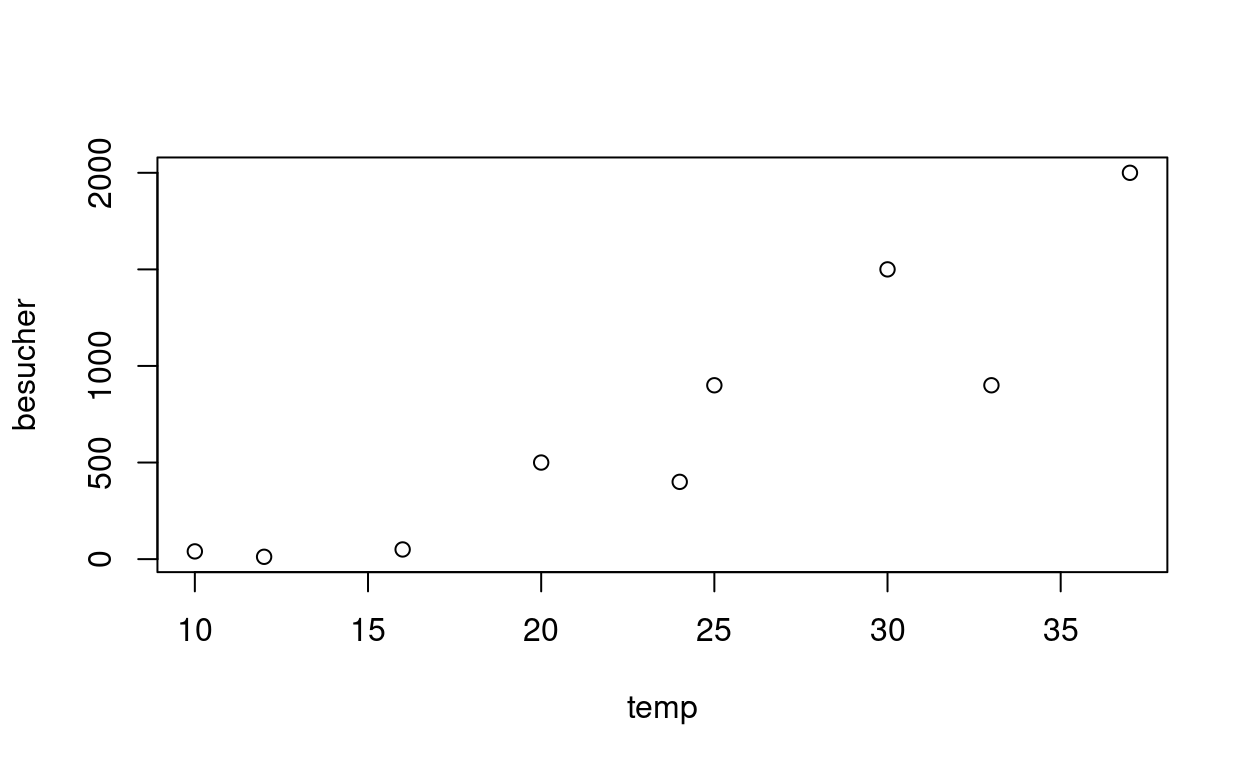
\includegraphics{solution_stat2.2_files/figure-latex/unnamed-chunk-2-1.pdf}

\begin{Shaded}
\begin{Highlighting}[]
\CommentTok{# definiert das Modell (vgl. Skript Statistik 2)}
\NormalTok{model <-}\StringTok{ }\KeywordTok{aov}\NormalTok{(tot_sold }\OperatorTok{~}\StringTok{ }\NormalTok{label_content, }\DataTypeTok{data =}\NormalTok{ df)}

\KeywordTok{summary.lm}\NormalTok{(model)}
\end{Highlighting}
\end{Shaded}

\begin{verbatim}
## 
## Call:
## aov(formula = tot_sold ~ label_content, data = df)
## 
## Residuals:
##      Min       1Q   Median       3Q      Max 
## -218.583  -39.938   -1.708   56.917  282.417 
## 
## Coefficients:
##                           Estimate Std. Error t value Pr(>|t|)    
## (Intercept)                1135.58      31.52   36.03   <2e-16 ***
## label_contentHot and Cold  -827.25      44.58  -18.56   <2e-16 ***
## label_contentPflanzlich   -1014.25      48.15  -21.07   <2e-16 ***
## label_contentPflanzlich+   -915.36      48.15  -19.01   <2e-16 ***
## label_contentVegetarisch   -652.50      44.58  -14.64   <2e-16 ***
## ---
## Signif. codes:  0 '***' 0.001 '**' 0.01 '*' 0.05 '.' 0.1 ' ' 1
## 
## Residual standard error: 109.2 on 49 degrees of freedom
## Multiple R-squared:  0.9257, Adjusted R-squared:  0.9196 
## F-statistic: 152.6 on 4 and 49 DF,  p-value: < 2.2e-16
\end{verbatim}

\begin{Shaded}
\begin{Highlighting}[]
\CommentTok{# überprüft die Modelvoraussetzungen}
\KeywordTok{par}\NormalTok{(}\DataTypeTok{mfrow =} \KeywordTok{c}\NormalTok{(}\DecValTok{2}\NormalTok{,}\DecValTok{2}\NormalTok{))}
\KeywordTok{plot}\NormalTok{(model)}
\end{Highlighting}
\end{Shaded}

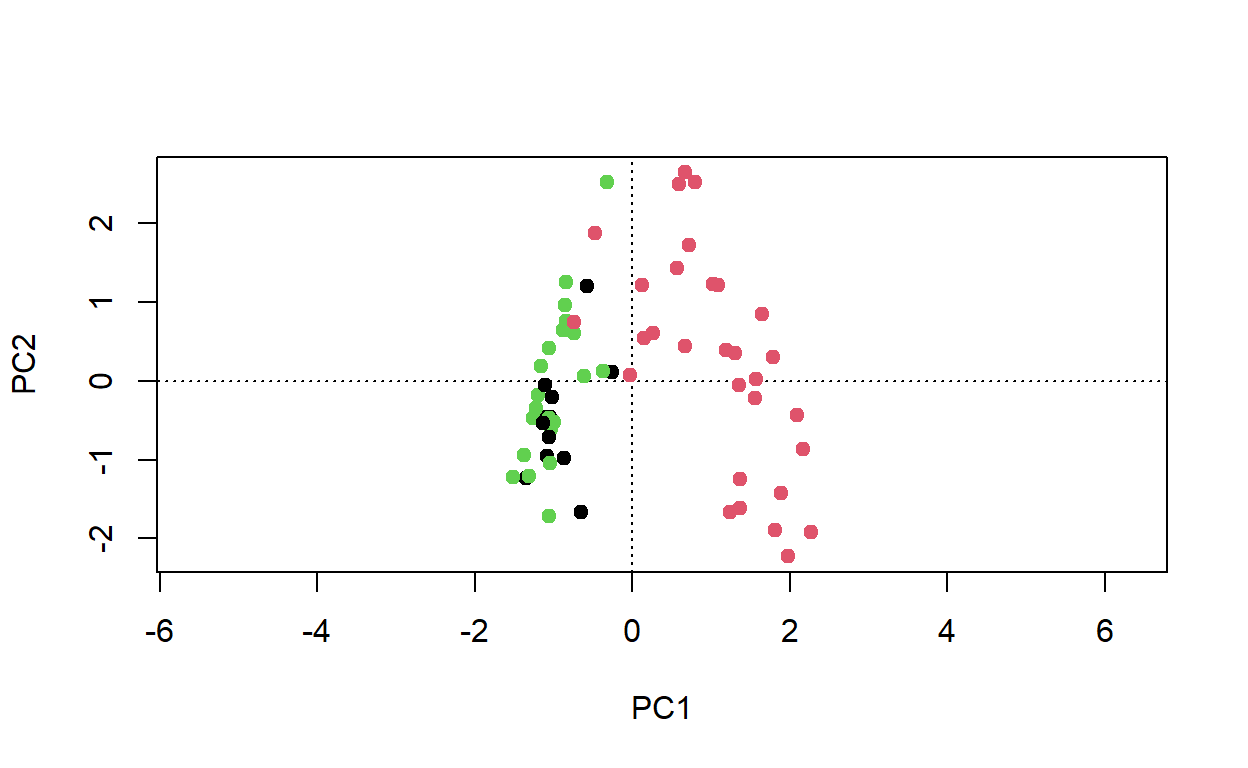
\includegraphics{solution_stat2.2_files/figure-latex/unnamed-chunk-2-2.pdf}
\\
{\textbf{Fazit}: Inspektion der Modellvoraussetzung zeigt klare
Verletzungen des Residuelplots (zeigt einen ``Trichter'', siehe Skript
Statistik 2), somit Voraussetzung der Homoskedastizität verletzt.
Mögliche nächste Schritte: * Menüinhalt ``Buffet'' aus der Analyse
ausschliessen, da sowieso kein richtiger Menüinhalt (aber
Informationsverlust) * Datentransformation * nicht-parametrischer Test.}
* ein glm Model (general linear model) mit einer poisson/quasipoisson
link Funktion (vgl. Skript Statistik 4), weitere Infos dazu
\href{https://www.ncbi.nlm.nih.gov/pmc/articles/PMC5869353/}{Link}

\begin{Shaded}
\begin{Highlighting}[]
\CommentTok{# überprüft die Voraussetzungen des Welch-Tests:}
\CommentTok{# Gibt es eine hohe Varianzheterogenität und ist die relative Verteilung der Residuen gegeben? (siehe Folien Statistik 2: Folie 18)}
\CommentTok{# Ja Varianzheterogenität ist gegeben, aber die Verteilung der Residuen folgt einem "Trichter", also keiner "normalen/symmetrischen" Verteilung um 0}
\CommentTok{# Daher ziehe ich eine Transformation der AV einem nicht-parametrischen Test vor}
\CommentTok{# für weitere Infos: https://data.library.virginia.edu/interpreting-log-transformations-in-a-linear-model/}
\NormalTok{model_log <-}\StringTok{ }\KeywordTok{aov}\NormalTok{(}\KeywordTok{log10}\NormalTok{(tot_sold) }\OperatorTok{~}\StringTok{ }\NormalTok{label_content, }\DataTypeTok{data =}\NormalTok{ df) }\CommentTok{# achtung hier log10, bei Rücktransformation achten}

\KeywordTok{par}\NormalTok{(}\DataTypeTok{mfrow =} \KeywordTok{c}\NormalTok{(}\DecValTok{2}\NormalTok{,}\DecValTok{2}\NormalTok{))}
\KeywordTok{plot}\NormalTok{(model_log) }\CommentTok{# scheint ok zu sein}
\end{Highlighting}
\end{Shaded}

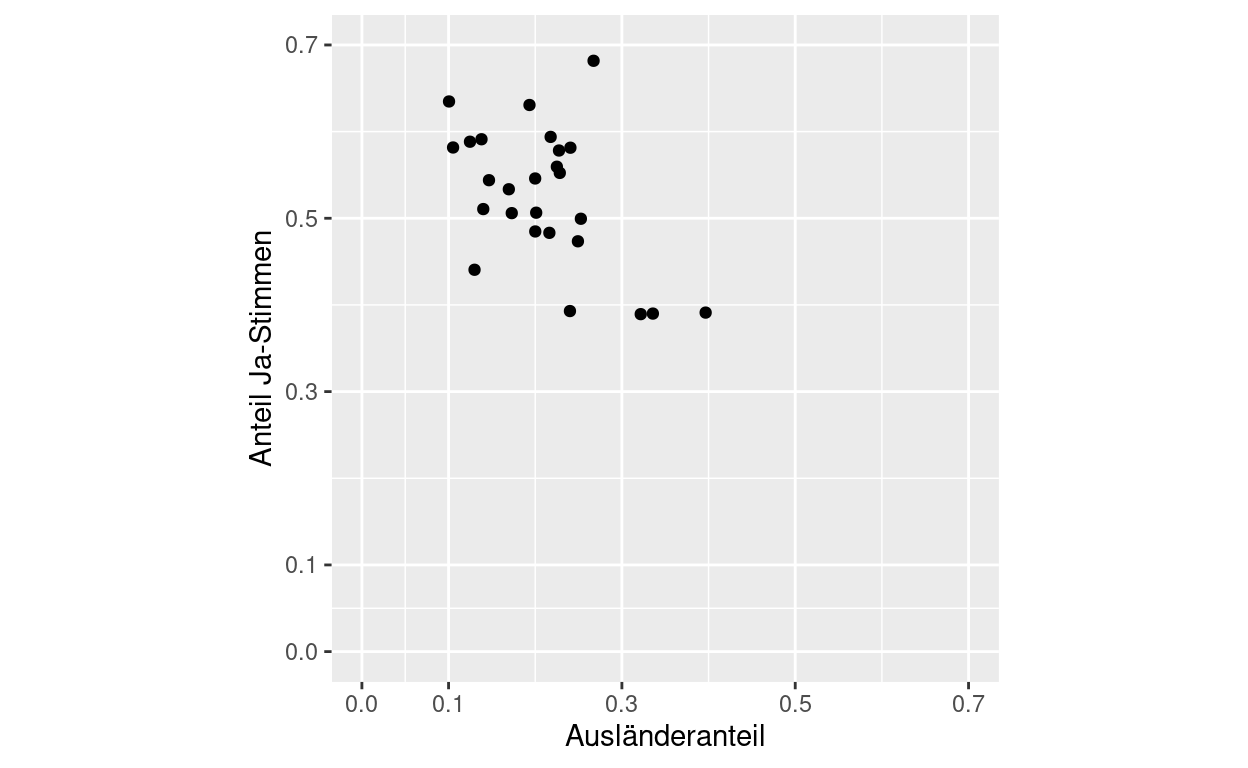
\includegraphics{solution_stat2.2_files/figure-latex/unnamed-chunk-3-1.pdf}

\begin{Shaded}
\begin{Highlighting}[]
\KeywordTok{summary.lm}\NormalTok{(model_log) }\CommentTok{# Referenzkategorie ist der Buffet-Inhalt}
\end{Highlighting}
\end{Shaded}

\begin{verbatim}
## 
## Call:
## aov(formula = log10(tot_sold) ~ label_content, data = df)
## 
## Residuals:
##      Min       1Q   Median       3Q      Max 
## -0.62985 -0.05056  0.00234  0.06539  0.21800 
## 
## Coefficients:
##                           Estimate Std. Error t value Pr(>|t|)    
## (Intercept)                3.04908    0.04048  75.321  < 2e-16 ***
## label_contentHot and Cold -0.56121    0.05725  -9.803 3.88e-13 ***
## label_contentPflanzlich   -0.99198    0.06184 -16.042  < 2e-16 ***
## label_contentPflanzlich+  -0.76602    0.06184 -12.388  < 2e-16 ***
## label_contentVegetarisch  -0.36893    0.05725  -6.444 4.82e-08 ***
## ---
## Signif. codes:  0 '***' 0.001 '**' 0.01 '*' 0.05 '.' 0.1 ' ' 1
## 
## Residual standard error: 0.1402 on 49 degrees of freedom
## Multiple R-squared:  0.8629, Adjusted R-squared:  0.8517 
## F-statistic: 77.12 on 4 and 49 DF,  p-value: < 2.2e-16
\end{verbatim}

\begin{Shaded}
\begin{Highlighting}[]
\KeywordTok{TukeyHSD}\NormalTok{(model_log) }\CommentTok{# (Statistik 2: Folien 9-11)}
\end{Highlighting}
\end{Shaded}

\begin{verbatim}
##   Tukey multiple comparisons of means
##     95% family-wise confidence level
## 
## Fit: aov(formula = log10(tot_sold) ~ label_content, data = df)
## 
## $label_content
##                                diff         lwr         upr     p adj
## Hot and Cold-Fleisch     -0.5612085 -0.72333441 -0.39908256 0.0000000
## Pflanzlich-Fleisch       -0.9919800 -1.16709603 -0.81686400 0.0000000
## Pflanzlich+-Fleisch      -0.7660203 -0.94113636 -0.59090433 0.0000000
## Vegetarisch-Fleisch      -0.3689328 -0.53105876 -0.20680691 0.0000005
## Pflanzlich-Hot and Cold  -0.4307715 -0.60588755 -0.25565551 0.0000001
## Pflanzlich+-Hot and Cold -0.2048119 -0.37992788 -0.02969584 0.0143708
## Vegetarisch-Hot and Cold  0.1922757  0.03014972  0.35440158 0.0126407
## Pflanzlich+-Pflanzlich    0.2259597  0.03875277  0.41316657 0.0107017
## Vegetarisch-Pflanzlich    0.6230472  0.44793117  0.79816320 0.0000000
## Vegetarisch-Pflanzlich+   0.3970875  0.22197149  0.57220353 0.0000005
\end{verbatim}

\begin{Shaded}
\begin{Highlighting}[]
\CommentTok{# Achtung Beta-Werte resp. Koeffinzienten sind nicht direkt interpretierbar}
\CommentTok{# sie müssten zuerst wieder zurück transformiert werden, hier ein Beispiel dafür:}
\CommentTok{# für Buffet}
\DecValTok{10}\OperatorTok{^}\NormalTok{model_log}\OperatorTok{$}\NormalTok{coefficients[}\DecValTok{1}\NormalTok{]}
\end{Highlighting}
\end{Shaded}

\begin{verbatim}
## (Intercept) 
##    1119.655
\end{verbatim}

\begin{Shaded}
\begin{Highlighting}[]
\CommentTok{# für Fleisch}
\DecValTok{10}\OperatorTok{^}\NormalTok{(model_log}\OperatorTok{$}\NormalTok{coefficients[}\DecValTok{1}\NormalTok{] }\OperatorTok{+}\StringTok{ }\NormalTok{model_log}\OperatorTok{$}\NormalTok{coefficients[}\DecValTok{2}\NormalTok{])}
\end{Highlighting}
\end{Shaded}

\begin{verbatim}
## (Intercept) 
##    307.5216
\end{verbatim}

\begin{Shaded}
\begin{Highlighting}[]
\CommentTok{# für Vegi}
\DecValTok{10}\OperatorTok{^}\NormalTok{(model_log}\OperatorTok{$}\NormalTok{coefficients[}\DecValTok{1}\NormalTok{] }\OperatorTok{+}\StringTok{ }\NormalTok{model_log}\OperatorTok{$}\NormalTok{coefficients[}\DecValTok{3}\NormalTok{])}
\end{Highlighting}
\end{Shaded}

\begin{verbatim}
## (Intercept) 
##    114.0523
\end{verbatim}

\textbf{Methoden}

Ziel war es, die Unterschiede in den wöchentlichen Verkaufszahlen pro
Menüinhalt aufzuzeigen. Da die Responsevariable (Verkaufszahlen)
metrisch und die Prädiktorvariable kategorial sind, wurde eine
einfaktorielle ANOVA gerechnet. Die visuelle Inspektion des Modells
zeigte insbesondere schwere Verletzungen der Homoskedastizität. Der
Boxplot bestätigt dieser Befund. Weil die Voraussetzungen schwer
verletzt sind, wurde eine log-Transformation der Responsevariable
vorgenommen. Anschliessend wurde erneut eine ANOVA gerechnet und die
Modelvoraussetzungen visuell inspiziert: Homoskedastizität und
Normalverteilung der Residuen sind gegeben.

\begin{center}\rule{0.5\linewidth}{\linethickness}\end{center}

\textbf{Ergebnisse}

Die Menüinhalte (Fleisch, Vegetarisch und Buffet) unterscheiden sich in
den wöchentlichen Verkaufszahlen signifikant (F(2,15) = 77.12, p
\textless{} .001). Die Abbildung 1 zeigt die wöchentlichen
Verkaufszahlen pro Menüinhalt.

\begin{figure}
\centering
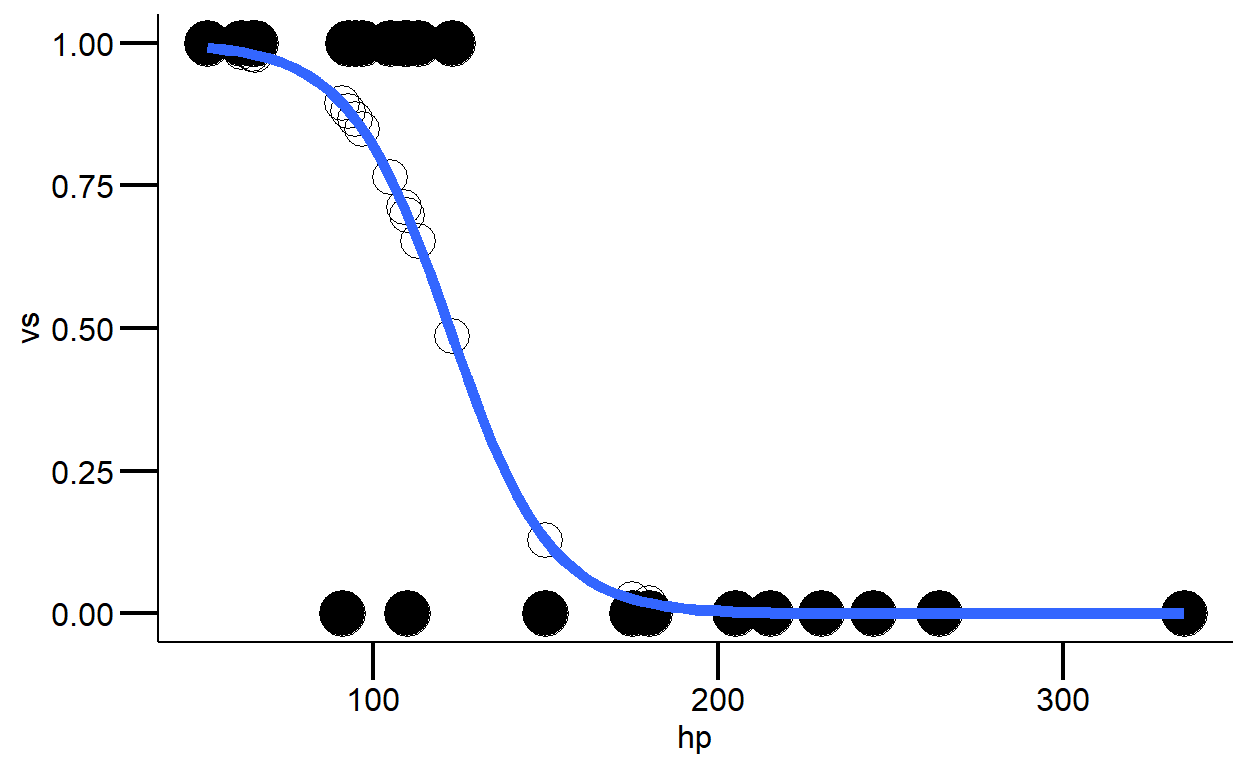
\includegraphics{solution_stat2.2_files/figure-latex/unnamed-chunk-4-1.pdf}
\caption{Die wöchentlichen Verkaufzahlen unterscheiden sich je nach
Menüinhalt stark. Das Modell wurde mit den log-tranformierten Daten
gerechnet.}
\end{figure}


\end{document}
